%-----------------------------------------------------------------------------------------
\clearpage
\section{Project Specification}
%-----------------------------------------------------------------------------------------
This part is the specification of the project which includes the features specification and technology choices to the software. The user features the system will also be stated. The project specification discussed in the initial document is modified and updated here as a section of the final dissertation.

\subsection{Data Characteristics}

Data is a major part of all visualisation, which along with user experience play an important role as "driving factor" with respect to the choice and attributes of the visualization method \cite{Laramee}. In this chapter, the data relevant to this project is analysed, including the type, size, format, and characteristics of data. Also, a description of data preprocessing will be discussed. 

The data sets used in this project come from a collection of 57 different German translations of \emph{Othello}, which is contributed by Dr. Tom Cheesman, from College of Arts and Humanities at Swansea University, working on a project in \cite{Tom2012}. To develop analytic tools and probe the translations in this corpus, the team digitalized 32 translation versions, with the formats being normalized, texts being segmented, speech by speech and line by line. The content of these 32 texts corresponds to Act1, Scene 3 of the English version of \emph{Othello} (1604) play as the base text. Based on this corpus, we are given 15 text files of German translation versions by Dr. Tom Cheesman for this project. And together with the base text in English, these 16 text sets are read and processed when implementing the project.All these files are encoded as UTF-8 when converting from .docx format to .txt format. The number of words in each document are different according to the genres of text data (327 words at maximum, and 214 words at minimum). Figure \ref{fig:dataExample} is a screen shot of the text data used in the project. All data has been segmented and cleaned
\begin{figure}[H]
	\centering    
	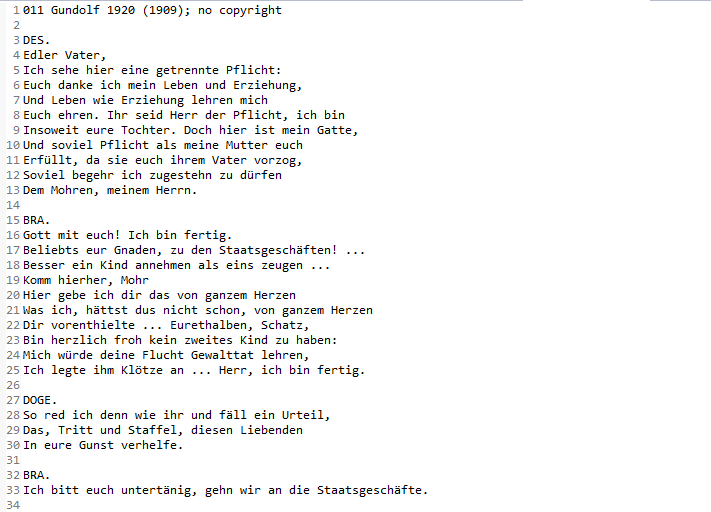
\includegraphics[scale=0.8]{Figs/Data-example}\\[1ex]
	\caption{A screen shot of text data used in this project.}
	\label{fig:dataExample}
\end{figure}
The text file is commonly used to store plain texts data. It is a simple text file format which can be worked with many programming languages, including Java. Choosing .txt file as the data set is owing to following reasons:

\begin{itemize}
	\item \textbf{} The aim of this project focuses on word processing, which requires computers to read text literally, without applying complicated data processing techniques.
	\item \textbf{} Since the text data sets in the corpus are stored in .docx format which is difficult to read directly from Java, it is easier and safer to convert the .docx format into .txt format.
	\item \textbf{} There exist methods in Java.io, a Java API, used to read .txt data directly from files.
	\item \textbf{} Apart from the basic and simple information (publication year and author) of each version, there is no need to obtain more information from the text. Additionally, because the data set in each version is not large, the computer can calculate the essential features of the data, in a short time, every time the program is ran. 
\end{itemize}


\subsection{Feature Specification}
This project is aimed at developing an interactive visualisation for a group of different text documents. The result of this visualisation should assist users in identifying and exploring the variations between these translation versions. The software has following features:
\begin{itemize}
	\item \textbf{} Provide an interactive visualisation system.
	\item \textbf{} Develop a user interface serves as a tool for users to select options.
	\item \textbf{} Read and store data from .txt files.
	\item \textbf{} Provide a parallel visualisation for comparing terms in different translation versions.
	\item \textbf{} Generate concordance view with frequency bars
	\item \textbf{} Add author and publish year as the title of each concordance.
	\item \textbf{} Provide a visualisation with scroll bars.
	\item \textbf{} Connect same words in each concordance applying coloured edge.
	\item \textbf{} Provide user option for scaling the visualisation.
	\item \textbf{} Scale the size of window.
	\item \textbf{} Generate a colour mapping view, and the colour represents the frequency of words.
	\item \textbf{} Render a user option for turning translations on and off.
	\item \textbf{} Create an English-German word translation index.
	\item \textbf{} Add user option: highlight the bar and connection when clicking single bar.
	\item \textbf{} Provide user option: highlight bars with same frequency when clicking a block in colour legend.
	\item \textbf{} Generate a Lemma and Frequency visualisation.
	\item \textbf{} Generate a Tf-Idf Visualisation.
	\item \textbf{} Generate a Lemma and Tf-Idf  Visualisation.
\end{itemize}
\subsection{Technology Choices}
According to the project specification and required features presented previously, the demonstration of technology choices is made in the following chapter.
\subsubsection{Programming language}
For the implementation of the software in this project, Java programming language is selected to develop the software. Java has known that it is an object-oriented language and class-based \cite{Gosling2014}. It is also simple enough to understand fast. With years of upgrading and improvement, it has been growing into a mature programming language. This also means using Java to develop software will have fewer mistakes and bugs when programming. There are also active communities on the internet, in which lots of people share useful ideas and resources of Java. In addition, due to the limitation of background which is not Computer Science, the author is more familiar with Java programming language.  

\subsubsection{Java Library}

\paragraph{Java Swing Library}
\paragraph[]{} The Java Swing Library is the tool we used in this project to generate GUI of the software. This is a free, cross-platform resource which is appropriate for using Java in implementing this project.

\paragraph{Stanford NLP Library}
\paragraph[]{} The Stanford NLP Library is attempted during we generate the lemma for English version text \cite{StanfordNLP}. This is a free and open source for Natural Language Processing. However, because this library has not provided German lemmatisation function, we adopted other solutions in this project.

\subsubsection{Other Techniques}

\paragraph{TreeTagger}
\paragraph[]{}TreeTagger, developed by Helmut Schmid at the Institute for Computational Linguistics of the University of Stuttgart \cite{TreeTagger}, is a tool for annotating text data and lemma information. It has been used to tag many languages including German.

\paragraph{Github}
\paragraph[]{} For source code backup requirement, the Github is adopted. The main software we used most is the GitKraken (See Figure \ref{fig:gitKraken}), which provides an interactive user interface to commit project. As a version control tool, the Github helps in organizing the development process of our software and in keeping an updated version of the software.

\begin{figure}[H]
	\centering    
	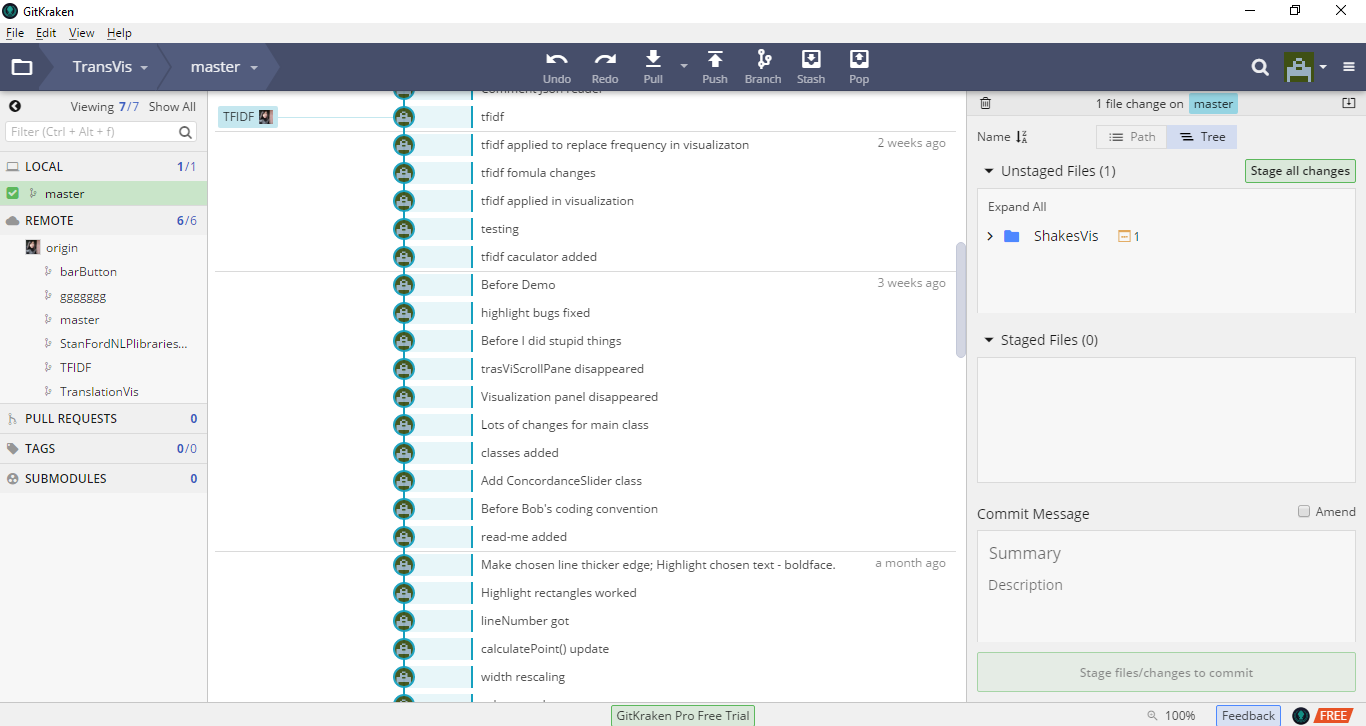
\includegraphics[scale=0.4]{Figs/GitKraken}\\[1ex]
	\caption{A screenshot for the user interface of GitKraken.}
	\label{fig:gitKraken}
\end{figure}

\paragraph{Dropbox}
\paragraph[]{} The Dropbox is another backup software which can be used to store data. We adopt this software to store our source data in the case that equipment is broken, or the website of Github is collapsed.
\textit{}
\paragraph{Eclipse and Visual Studio Code}
\paragraph[]{} Eclipse and Visual Studio Code are tools we used in this project for Java programming. The Eclipse is the main tool to program in Java, while the Visual Studio Code serves as a backup software in the case that Eclipse is collapsed. 

\paragraph{Notepad++}
\paragraph[]{}The Notepad++ is a free and useful tool for source code editing. It also supports editing files in many kinds of format. In this project, we adopt Notepad++ to encode data during Data Processing phase.
